%%=============================================================================
%% Linux server concepten
%%=============================================================================

\chapter{\IfLanguageName{dutch}{Linux server concepten}{Linux server concepts}}%
\label{ch:linux-server-concepten}

\section{Inleiding}
\label{linux_inleiding}

Om ons te helpen bij het maken van een configuratie-inventaris van een Linux systeem, moeten we verschillende aspecten van Linux in acht nemen.
Door enkele basisconcepten te kennen over de verschillende componenten en functies van een Linux systeem en de beschikbare ondersteunende tools, is het veel eenvoudiger om te bepalen wat we in onze inventaris moeten opnemen en wat niet.
In dit hoofdstuk worden enkele basisbegrippen van Linux uitgelegd, zoals wat het is en wat er deel van uitmaakt, enz.

\section{Het Linux besturingssysteem}
\label{linux_linux_besturingssysteem}

Een besturingsysteem is de software die applicaties toe laat om te communiceren met de hardware van een computer.
Vaak als we spreken over besturingssystemen, denken we aan Windows, macOS of Linux.
Echter is Linux hier een buitenbeentje, aangezien het niet een besturingssysteem is, maar een kernel.
De taak van de kernel is om de hardware van een computer te beheren en de software die op de computer draait te ondersteunen.

De kernel is het hart van een Linux-systeem, en is verantwoordelijk voor het beheer van de hardware van de computer, zoals de CPU, het geheugen, de opslag en de netwerkinterfaces.
Echter wanneer we spreken over een Linux-systeem, bedoelen we vaak de bundel van software die samen met de kernel wordt geleverd, zoals de GNU core-utils, de shell en de grafische interface.
Deze bundeling van software gaan we vaak een Linux-distributie noemen, of ook wel een distro genoemd.
Enkele bekende Linux-distributies zijn Debian, Ubuntu, Fedora en RHEL.

Een typisch Linux-systeem bestaat uit verschillende lagen, zoals te zien is in figuur~\ref{fig:linux-system-structure}.
De user space is diegene waar de gebruiker het meeste mee in contact komt, hier draaien de applicaties en de shell.
Applicaties hebben beperkte rechten, zo kunnen ze zelf geen hardware aanspreken, of aansturen.
Dit moet gebeuren door de Application Programming Interface (API) die de kernel aanbiedt, die system calls doet naar de kernel space, wat te zien is in figuur~\ref{fig:linux-system-structure}~\autocite{mauerer2008linux}.

\begin{figure}[h!]
    \begin{center}
        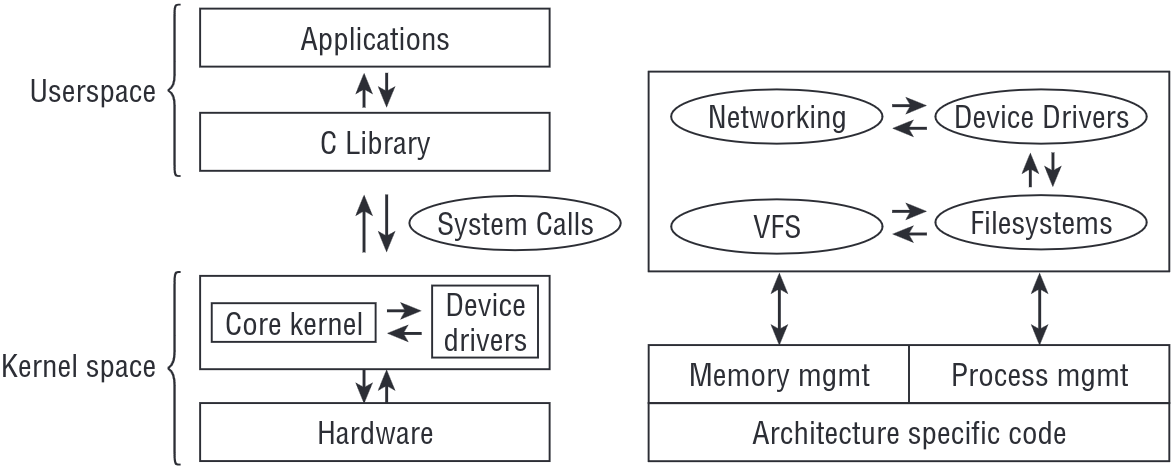
\includegraphics[width=\textwidth]
        {./graphics/linux/kernel-structure.png}
        \caption{\label{fig:linux-system-structure}Structuur van een typisch Linux-systeem~\autocite{mauerer2008linux}}
    \end{center}
\end{figure}

De Linux-kernel is wat we noemen een monolithische kernel, wat wil zeggen dat het een enkele grote binary is die alle functionaliteit bevat.
Dit houdt in dat alle subsystemen van de kernel, zoals het bestandssysteem, het geheugenbeheer en de netwerkstack, in dezelfde binary zitten.
Echter is de kernel wel modulair, wat wil zeggen dat we modules kunnen laden en lossen in de kernel, zonder dat we de kernel zelf moeten hercompileren.
Deze modules kunnen voor verschillende doeleinden worden gebruikt, zoals het toevoegen van ondersteuning voor nieuwe hardware, het beveiligen van het systeem met SELinux of AppArmor, of het toevoegen van nieuwe functionaliteit aan de kernel~\autocite{hypponen2021securing}.
Een voorbeeld van een module is \texttt{vboxdrv}, die nodig is om VirtualBox te kunnen gebruiken op een Linux-systeem.

\subsection{Applicatie beheer}
\label{linux_applicatie_beheer}

\subsubsection{Packaging systemen}
\label{linux_packaging_systemen}

Er bestaan vandaag de dag duizenden Linux-distributies die elk hun eigen manier van applicatiebeheer hebben.
Deze diversiteit komt tot uiting in de manier waarop ze hun pakketten beheren.
Toch kunnen de meeste van deze systemen grofweg worden ingedeeld in twee hoofdcategorie\"en: RHEL-gebaseerde systemen en Debi-\ an-gebaseerde systemen.

RHEL-gebaseerde systemen maken gebruik van het Red Hat Package Manager (RPM) systeem, terwijl Debian-gebaseerde systemen vertrouwen op het Debian Package Manager (DPKG) systeem.
Deze twee packaging-systemen vormen de ruggengraat van het applicatiebeheer op hun respectievelijke distributies.
Een beknopt overzicht van de distributies die deze packaging-systemen gebruiken, wordt gepresenteerd in tabel~\ref{table:packaging-systems}.

\begin{table}[!h]
    \begin{center}
        \begin{tabular}{ c c  }
            \hline
                Packaging systeem & Distributies\\ [0.5ex] 
            \hline
            Debian Package Manager (DPKG)     & Debian, Ubuntu, Linux Mint \\
            Red Hat Package Manager (RPM)     & RHEL, Fedora, openSUSE \\
        \end{tabular}
    \end{center}
    \caption{Overzicht van de verschillende packaging systemen en de distributies die ze gebruiken~\autocite{shotts2019linux}.}
    \label{table:packaging-systems}
\end{table}

Hoewel RHEL- en Debian-gebaseerde distributies de dominante spelers zijn, zijn er enkele uitzonderingen op deze regel.
Sommige distributies hebben hun eigen unieke package manager, zoals Arch Linux met pacman, of Gentoo met Portage.
Niettemin behoren de meeste andere distributies tot de RHEL- of Debian-families, en maken ze gebruik van RPM of DPKG voor hun applicatiebeheer.

\subsubsection{Package managers}
\label{linux_package_managers}

De package manager speelt een essenti\"ele rol bij het beheer van software op een systeem.
Het stelt gebruikers in staat om software te installeren, te verwijderen en bij te werken, en zorgt ervoor dat eventuele afhankelijkheden van software adequaat worden beheerd.
Bovendien is versiebeheer een belangrijk aspect van package managers, waarbij de juiste versie van de software wordt ge\"installeerd en up-to-date wordt gehouden door de package manager.

We kunnen de package manager ook inzetten om een lijst van ge\"installeerde softwarepakketten te bekijken, iets wat we later in dit werk zullen gebruiken om een configuratie-inventaris te maken.
Op Debian-gebaseerde systemen kunnen we dit bijvoorbeeld doen door het commando \texttt{apt list --installed} als de root-gebruiker uit te voeren.
Als alternatief kan men ook \texttt{dpkg-query -l} gebruiken, wat ons toelaaat om query's uit te voeren op de DPKG-database, zoals te zien in listing~\ref{lst:dpkg-query}.

\begin{listing}
  \begin{minted}[linenos,tabsize=4,breaklines]{console}
vagrant@srv1:~$ sudo dpkg-query -Wf '"${Package}" "${Version}" "${Source}"\n'
"adduser" "3.134" ""
"apparmor" "3.0.8-3" ""
"apt" "2.6.1" ""
"apt-listchanges" "3.24" ""
"apt-utils" "2.6.1" "apt"
"base-files" "12.4+deb12u5" ""
"base-passwd" "3.6.1" ""
"bash" "5.2.15-2+b2" "bash (5.2.15-2)"
"bash-completion" "1:2.11-6" ""
"bind9-dnsutils" "1:9.18.24-1" "bind9"
[...]
  \end{minted}
  \caption{Uitvoer van het \texttt{dpkg-query} commando om een lijst van ge\"installeerde softwarepakketten te tonen.}
  \label{lst:dpkg-query}
\end{listing}

\subsubsection{Repositories}
\label{linux_repositories}

De meeste package managers halen hun softwarepakketten uit zogenaamde repositories, die dienen als centrale opslagplaatsen voor gebruikers om softwarepakketten te downloaden en te installeren.
Deze repositories bevatten vaak duizenden softwarepakketten die allemaal beheerd kunnen worden door de package manager~\autocite{shotts2019linux}.

Dergelijke repositories worden doorgaans beheerd door de distributie zelf, maar het komt ook vaak voor dat ge\"interesseerde gebruikers bijdragen aan het onderhouden van de pakketten in de repository.
Bovendien bieden de meeste package managers de flexibiliteit om extra repositories toe te voegen, waardoor gebruikers software kunnen installeren die niet beschikbaar is in de standaard repositories.

Een voorbeeld hiervan is Ubuntu, dat gebruikers de mogelijkheid biedt om PPAs toe te voegen, wat staat voor Personal Package Archives.
Deze PPAs worden onderhouden door individuele gebruikers en bevatten software die niet in de standaard repositories van Ubuntu te vinden is.
Een vergelijkbare functionaliteit wordt aangeboden door Fedora met COPR, wat staat voor Cool Other Package Repositories.

\subsection{Bestandssystemen}
\label{linux_bestandssystemen}

Het bestandssysteem is een belangrijk onderdeel van een Linux-systeem, en is verantwoordelijk voor het makklijk toegang verlenen tot opslagmedia, zoals Hard Drive Disks (HDD's), Solid State Drive (SSD's) en USB-sticks.
Naast het toegang verlenen tot opslagmedia, is het bestandssysteem ook verantwoordelijk voor het beheren van bestanden en directories, en het toekennen van permissies aan deze bestanden en directories.
Dit gebeurt door middel van twee verschillende delen, de collectie van bestanden en directories, en de metadata die hieraan is gekoppeld.
Deze metadata bevat informatie zoals de eigenaar van het bestand, de groep waartoe het bestand behoort, de permissies die zijn toegekend aan het bestand en de timestamps van de creatie, wijziging en toegang van het bestand.
De verzamelnaam voor deze metadata worden ook wel de bestandsattributen genoemd~\autocite{silberschatz2013os}
Verschillende bestandssystemen kunnen worden gebruikt op een Linux-systeem, zoals ext4, xfs, btrfs en zfs.

\begin{listing}
  \begin{minted}[linenos,tabsize=4,breaklines]{console}
[root@fedorable ~]# tree -L 1 /
/
├── afs
├── bin -> usr/bin
├── boot
├── dev
├── etc
├── home
├── lib -> usr/lib
├── lib64 -> usr/lib64
├── lost+found
├── media
├── mnt
├── opt
├── proc
├── root
├── run
├── sbin -> usr/sbin
├── srv
├── sys
├── tmp
├── usr
└── var
  \end{minted}
  \caption{Uitvoer van het \texttt{tree}-commando op een Fedora Linux-systeem om de hi\"erarchische structuur van het Linux-bestandssysteem te tonen.}
  \label{lst:linux-root-dir-structure}
\end{listing}

Linux maakt gebruik van een hi\"erarchisch bestandssysteem, wat wil zeggen dat bestanden en directories worden georganiseerd in een boomstructuur, zoals te zien is in listing~\ref{lst:linux-root-dir-structure}.
Startend vanuit de root directory, die wordt aangeduid met een schuine streep (\texttt{/}), worden bestanden en directories georganiseerd in verschillende niveaus van subdirectories.
Elke directory binnen de root directory kan op zijn beurt bestanden en subdirectories bevatten, met elk hun eigen doel en functie.
Zo heeft de \texttt{etc} directory, staande voor ``et cetera'', de configuratiebestanden voor verschillende softwarepakketten, terwijl de \texttt{bin} directory de binaries bevat die nodig zijn om het systeem te laten functioneren~\autocite{linuxfoundation-filesystem}.

\subsection{Gebruikers en groepen}
\label{linux_gebruikers_groepen}

De Linux-kernel biedt ondersteuning voor het gelijktijdig beheren van meerdere gebruikers, waarbij elke gebruiker wordt onderscheiden aan de hand van hun User ID (UID).
Een gebruiker vertegenwoordigt een entiteit die toegang heeft tot het systeem en de mogelijkheid heeft om bestanden en directories te maken en te bewerken.
Het concept van gebruikers is essentieel om de toegangsrechten en permissies op het systeem te beheren, waardoor een gecontroleerde en veilige omgeving wordt gecre\"eerd.
In veel gevallen heeft elk proces in de user-space zijn eigen gebruiker, die de rechten en permissies van dat proces bepaalt~\autocite{ward2021linux}.

Linux-systemen bevatten typisch meerdere gebruikersaccounts, met als eerste de superuser, die wordt ge\"identificeerd door een UID van 0, zoals weer te geven in listing~\ref{lst:linux-root-id}, en alle rechten heeft op het systeem.
Daarnaast kunnen gebruikersaccounts worden onderverdeeld in twee categorie\"en: systeemgebruikers en normale gebruikers.
Systeemgebruikers hebben doorgaans een UID lager dan 1000 en worden vaak gebruikt voor het draaien van services, zoals een Apache-webserver of een MySQL-database.
Aan de andere kant worden normale gebruikers ge\"identificeerd door een UID hoger dan 1000 en worden ze gebruikt door individuen die het systeem actief gebruiken, zoals systeembeheerders. Een voorbeeld van de uitvoer van het \texttt{id} commando voor een normale gebruiker is te zien in listing~\ref{lst:linux-anton-id}.

\begin{listing}
  \begin{minted}[linenos,tabsize=4,breaklines]{console}
[root@fedorable ~]# id
uid=0(root) gid=0(root) groups=0(root)
  \end{minted}
  \caption{Uitvoer van het \texttt{id}-commando voor de superuser, waarop we kunnen zien dat de gebruiker een UID van 0 heeft, een GID van 0 heeft en lid is van de groep \texttt{root}.}
  \label{lst:linux-root-id}
\end{listing}

\begin{listing}
  \begin{minted}[linenos,tabsize=4,breaklines]{console}
[anton@fedorable ~]$ id
uid=1000(anton) gid=1000(anton) groups=1000(anton),10(wheel)
  \end{minted}
  \caption{Uitvoer van het \texttt{id}-commando voor een normale gebruiker, waarop we kunnen zien dat de gebruiker een UID van 1000 heeft, een GID van 1000 heeft en lid is van de groepen \texttt{anton} en \texttt{wheel}.}
  \label{lst:linux-anton-id}
\end{listing}

Naast individuele gebruikers kunnen gebruikers ook worden gegroepeerd in groepen, die een verzameling van gebruikers vertegenwoordigen met dezelfde rechten en permissies.
Groepen worden ook ge\"identificeerd door een unieke Group ID (GID), waarmee ze kunnen worden ge\"identificeerd en beheerd binnen het systeem.
Het gebruik van gebruikers en groepen biedt een gestructureerde manier om de toegangscontrole en beveiliging op een Linux-systeem te beheren, waardoor een geordende en veilige werkomgeving wordt bevorderd.
Zo hebben gebruikers die tot de wheel groep behoren op RHEL-gebaseerde systemen, zoals Fedora en AlmaLinux, de mogelijkheid om root-privileges te verkrijgen door het uitvoeren van het \texttt{sudo} commando.

\begin{table}[!h]
    \begin{adjustbox}{width=1\textwidth}
        \begin{tabular}{ c c  }
            \hline
                Afkorting & Betekenis\\ [0.5ex] 
            \hline
                Gebruikers & Een entiteit die toegang heeft tot het systeem en bestanden en directories kan maken en bewerken. \\
                Groepen    & Een verzameling van gebruikers die dezelfde rechten en permissies hebben. \\
                UID        & Staande voor User ID, is een uniek nummer dat aan een gebruiker wordt toegekend. \\
                GID        & Staande voor Group ID, is een uniek nummer dat aan een groep wordt toegekend. \\
        \end{tabular}
    \end{adjustbox}
    \caption{Overzicht van terminologie voor gebruikers en groepen.}
    \label{table:user-group-terminology}
\end{table}

Het \texttt{sudo} commando zal natuurlijk enkel werken als de gebruiker die het commando uitvoert, is toegevoegd aan de correcte groep in de \texttt{/etc/sudoers} file.
Als alternatief kan men ook een bestand dat bepaalde regels bevat aanmaken in de \texttt{/etc/sudoers.d/} directory, zoals te zien in listing~\ref{lst:linux-sudoers}.
Dit bestand bevat de verschillende regels die bepalen welke gebruikers en groepen root-privileges kunnen verkrijgen door het uitvoeren van het \texttt{sudo} commando.
Alsook wat ze kunnen uitvoeren, zo kan men bijvoorbeeld specifi\"eren dat een bepaalde gebruiker geen wachtwoord moet ingeven bij het uitvoeren van het \texttt{sudo} commando in combinatie met een bepaald commando.
Een voorbeeld van een \texttt{sudo}-regel is te zien in listing~\ref{lst:linux-sudoers}.

\begin{listing}
  \begin{minted}[linenos,tabsize=4,breaklines]{console}
[root@fedorable ~]# cat /etc/sudoers.d/anton
anton    ALL=(ALL)    NOPASSWD: /usr/bin/dnf
  \end{minted}
  \caption{Uitvoer van het \texttt{cat}-commando dat de inhoud van het bestand \texttt{/etc/sudoers.d/anton} laat zien. Hieruit blijkt dat de gebruiker \texttt{anton} root-privileges heeft voor het uitvoeren van het \texttt{dnf}-commando en geen wachtwoord hoeft in te voeren bij dit commando.}
  \label{lst:linux-sudoers}
\end{listing}

\subsection{Taakbeheer}
\label{linux_taakbeheer}

Services en processen vormen de ruggengraat van een Linux-systeem, waarbij ze cruciale taken uitvoeren en resources beheren om de algehele functionaliteit te ondersteunen.
Het correct beheren van deze services en processen is van vitaal belang voor de stabiliteit, prestaties en beveiliging van het systeem.

In dit gedeelte zullen we dieper ingaan op twee belangrijke aspecten van het beheer van services en processen op een Linux-systeem: systemd en cronjobs.

\subsubsection{Systemd}
\label{linux_systemd}

Systemd fungeert als een init-systeem op vele Linux-systemen, waardoor het mogelijk is om services te starten, stoppen en beheren als een user-space daemon tijdens het opstartproces.
In vergelijking met zijn voorgangers, zoals SysVinit en Upstart, biedt systemd aanzienlijk meer functionaliteit en wordt het vaak ingezet als een uitgebreide systeem- en servicebeheerder~\autocite{ward2021linux}.

Een van de krachtige kenmerken van systemd is het gebruik van unit files, die de configuratie van verschillende eenheden, zoals services, timers, sockets, devices en mount points, bevatten.
Hierdoor kunnen beheerders niet alleen services beheren, maar ook andere types eenheden.
Een overzicht van enkele veelgebruikte unit types wordt weergegeven in tabel~\ref{table:sytemd_unit_types}.

\begin{table}[!h]
    \begin{center}
        \begin{tabular}{ c c }
            \hline
                Unit type & Omschrijving \\ [0.5ex] 
            \hline
                Service & Een service die op de achtergrond draait en een bepaalde taak uitvoert. \\
                Timer   & Een timer die periodiek een service activeert. \\
                Device  & Een apparaat dat door het systeem wordt beheerd. \\
                Mount   & Een mount point voor een bestandssysteem. \\
        \end{tabular}
    \end{center}
    \caption{Overzicht van veelvoorkomende unit types in systemd.}
    \label{table:sytemd_unit_types}
\end{table}

Bovendien biedt systemd een mechanisme om afhankelijkheden tussen services te definiëren, waardoor het mogelijk is om complexe opstartvolgordes en -vereisten te beheren.
Met opties zoals \texttt{requires}, \texttt{wants}, \texttt{before} en \texttt{after} kunnen beheerders nauwkeurig aangeven welke services afhankelijk zijn van elkaar en in welke volgorde ze moeten worden gestart.
Dit draagt bij aan de fouttolerantie en consistentie van het systeem~\autocite{ward2021linux}.

Beheerders hebben de mogelijkheid om aangepaste unit files te maken en te bewerken in de \texttt{/etc/systemd/system/} of \texttt{/usr/lib/systemd/system/} directories, waardoor ze volledige controle hebben over de configuratie van services en andere eenheden~\autocite{ward2021linux}.

\subsubsection{Cronjobs}
\label{linux_cronjobs}

Cronjobs zijn geautomatiseerde taken die periodiek worden uitgevoerd op een Linux-systeem, zoals het maken van back-ups, het uitvoeren van systeemupdates of het genereren van rapporten.
Het zorgt ervoor dat we onafhankelijk van het progamma, op een bepaald tijdstip of interval, een bepaalde taak kunnen uitvoeren.
Dit gebruikmakende van de \texttt{cron} daemon, die de cronjobs beheert en uitvoert op de achtergrond.

Men kan cronjobs defini\"eren door middel van cron-tabellen, die de configuratie van de cronjobs bevatten.
Deze tabellen worden opgeslagen in de \texttt{/etc/cron.d/} directory, en kunnen worden bewerkt met behulp van de \texttt{crontab} commando~\autocite{ward2021linux}.

Een typische cron-tabel bestaat uit vijf velden, die de minuut, het uur, de dag van de maand, de maand en de dag van de week aangeven waarop de taak moet worden uitgevoerd.
Na de tijdvelden volgt het commando dat moet worden uitgevoerd, zoals te zien is in figuur~\ref{fig:cronjob-structure}, waar de structuur van een cron-tabel wordt weergegeven~\autocite{ward2021linux}.

\begin{figure}[h!]
    \begin{center}
        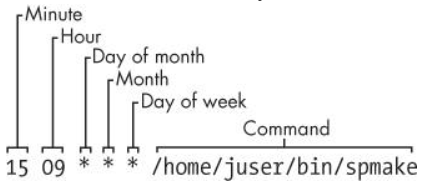
\includegraphics[width=200pt]
        {./graphics/linux/cronjob-structure.png}
        \caption{\label{fig:cronjob-structure}Structuur van een cron-tabel~\autocite{ward2021linux}.}
    \end{center}
\end{figure}

\section{Linux server beveiliging}
\label{linux_server_beveiliging}

Met de continue groei van het internet en de toenemende afhankelijkheid van digitale technologie, is het van cruciaal belang om de beveiliging van systemen te waarborgen.
Linux-servers zijn geen uitzondering en moeten worden beschermd tegen een breed scala aan bedreigingen, zoals denail-of-service (DoS), datalekken, enz.
In dit gedeeelte zullen we twee fundamentele concepten van Linux-serverbeveiliging bespreken: de firewall en SELinux.

\subsection{Firewall}
\label{linux_firewall}

Een veelgebruikte manier om een computernetwerk te beschermen van ongewenst verkeer is het gebruik van een firewall.
Dit is een fundamenteel onderdeel van cyberbeveiliging voor elke systeem, waaronder ook Linux-servers.
Zo kunnen firewalls voor verschillende doeleinden worden ingezet, zoals beschreven door van den Berg~\autocite{vandenberg}:

\begin{itemize}
    \item Het blokkeren of beperken van inkomend verkeer, zodat externe systemen niet zomaar verbinding kunnen maken met een server.
    \item Het blokkeren of beperken van uitgaand verkeer, om te voorkomen dat gevoelige gegevens het netwerk verlaten.
    \item Het vereisen van authenticatie om bepaalde diensten te gebruiken. Bij niet-toegestane directe verbindingen moeten gebruikers zich eerst identificeren bij de firewall, bijvoorbeeld door een gebruikersnaam en wachtwoord in te voeren.
    \item Het fungeren als proxy. Wanneer directe verbindingen naar buiten toe niet zijn toegestaan, kan de firewall worden ingeschakeld als proxy die het verkeer doorstuurt naar de bestemming.
\end{itemize}

Op Red Hat Enterprise Linux (RHEL) en zijn afgeleiden, zoals Fedora, wordt de firewall ge\"implementeerd met behulp van \texttt{firewalld}, een dynamisch beheerde firewall die het beheer van regels en zones vereenvoudigt.
Het laat ons niet alleen toe om regels te gaan defini\"eren op poort niveau, maar ook op basis van services, zoals SSH (Secure Shell), en deze toe te passen op specifieke zones, zoals de publieke zone~\autocite{dakic2022linux}.
De volledige architectuur van \texttt{firewalld} is te zien in figuur~\ref{fig:firewalld-architecture}.

\begin{figure}[h!]
    \begin{center}
        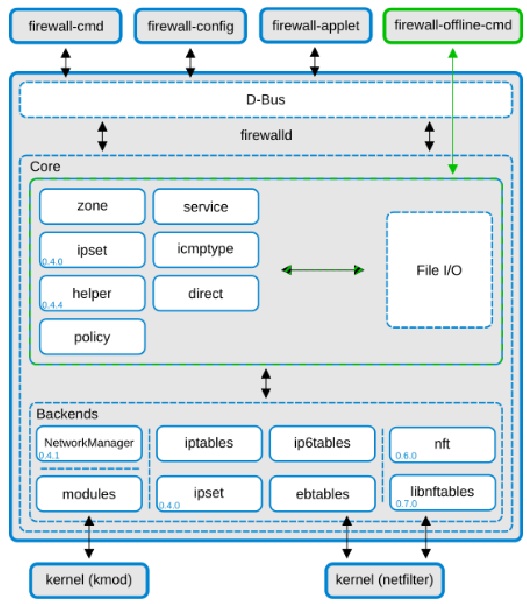
\includegraphics[width=200pt]
        {./graphics/linux/firewalld-architecture.png}
        \caption{\label{fig:firewalld-architecture}Architectuur van \texttt{firewalld}~\autocite{dakic2022linux}.}
    \end{center}
\end{figure}

Firewalld fungeert echter slechts als een frontend voor \texttt{nftables}~\autocite{dakic2022linux}, een framework dat de netfilter-module van de Linux-kernel vervangt.
Het is ontworpen om de complexiteit van \texttt{iptables} te verminderen.
Zowel \texttt{nftables} als \texttt{iptables} zijn onderdeel van de Linux-kernel, waar ze op kernelniveau netwerkpakketten evalueren aan de hand van de gedefinieerde regels~\autocite{ward2021linux}.

\subsection{Security Enhanced Linux}
\label{linux_selinux}

Security Enhanced Linux, of SELinux, biedt een geavanceerd beveiligingsframework bovenop de standaard Discretionary Access Control (DAC) implementatie van Linux.
DAC vertrouwt namelijk op gebruikers, groepen, en andere rechten om het beveiligingsbeleid van het systeem te bepalen, wat granulariteit mist.

Het is een extra beveiligingslaag die wordt toegevoegd aan de Linux-kernel en standaard aanwezig is op RHEL-gebaseerde systemen.
Echter kan het ook worden ge\"implementeerd op andere Linux-distributies, zoals Debian, maar is het niet standaard ge\"installeerd.

SELinux, of Security Enhanced Linux, voegt een extra laag van beveiliging toe aan Linux-systemen door middel van een Mandatory Access Control (MAC) model, bovenop het standaard Discretionary Access Control (DAC) systeem.
Het onderscheidt zich door unieke beveiligingslabels toe te voegen aan bestanden, processen en andere objecten op het systeem, waardoor het zich richt op beveiligingseigenschappen en abstractie biedt van systeemniveau-details.
Belangrijke elementen van SELinux contexten omvatten gebruiker, rol, type en beveiligingsniveau, waarbij type-informatie cruciaal is voor het handhaven van het beleid.
Deze types, zoals \texttt{httpd\_t} voor de webserver en \texttt{httpd\_sys\_content\_t} voor webserverbestanden, specificeren toegestane interacties tussen processen en bronnen~\autocite{selinux-rhel8}.

SELinux beleidsregels maken gebruik van deze contexten om toegang te beperken en te reguleren.
Bijvoorbeeld, de webserver Apache (\texttt{httpd\_t}) krijgt expliciete toegang tot bestanden in \texttt{/var/www/html/} (\texttt{httpd\_sys\_content\_t}) door middel van een beleidsregel.
Toegang tot andere mappen/ zoals \texttt{/data/mysql/}, wordt echter standaard geweigerd, tenzij specifiek aangegeven, zoals te zien is in figuur~\ref{fig:sleinux-example}~\autocite{selinux-rhel8}.
Deze strikte controle, zelfs in het geval van een gecompromitteerd proces zoals Apache, verhoogt de systeemveiligheid aanzienlijk, waardoor SELinux een krachtig instrument is voor het beveiligen van Linux-systemen.

\begin{figure}[h!]
    \begin{center}
        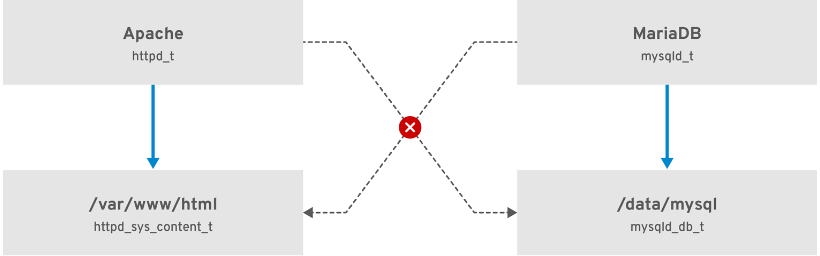
\includegraphics[width=300pt]
        {./graphics/linux/selinux-example.png}
        \caption{\label{fig:sleinux-example}Voorbeeld dat de werking van SELinux illustreert. De Apache-webserver kan enkel bestanden aanspreken die zijn gelabeld met het \texttt{httpd\_sys\_content\_t} label, terwijl de MariaDB-database enkel bestanden kan aanspreken die zijn gelabeld met het \texttt{mysqld\_db\_t} label~\autocite{selinux-rhel8}.}
    \end{center}
\end{figure}

\subsection{AppArmor}
\label{linux_apparmor}

In het voorgaande gedeelte is SELinux besproken als een beveiligingsframework dat een Mandatory Access Control (MAC) model implementeert.
Maar SELinux is niet de enige oplossing beschikbaar voor Linux-systemen.
Op Debian-gebaseerde systemen wordt vaak AppArmor gebruikt als een alternatief beveiligingsframework dat vergelijkbare functionaliteit biedt.

AppArmor, wat staat voor Application Armor, is ontworpen om applicaties te beschermen tegen ongeautoriseerde toegang tot het systeem.
Het bereikt dit door het isoleren van onbetrouwbare applicaties en het beperken van hun toegang tot bestanden, directories en andere bronnen.
Deze beperkingen worden ge\"implementeerd via profielen, die de toegestane interacties tussen applicaties en bronnen specificeren~\autocite{gruenbacher2007apparmor}.
Deze profielen worden opgeslagen in de \texttt{/etc/apparmor.d/} directory en kunnen worden aangepast om de beveiliging van het systeem te configureren~\autocite{apparmor-ubuntu}.
Het is echter belangrijk op te merken dat AppArmor zich beperkt tot deze profielen en niet de uitgebreide beveiligingsmogelijkheden biedt die SELinux biedt.

In tegenstelling tot SELinux maakt AppArmor geen gebruik van labels om toegang te beperken, maar gebruikt het paden.
Dit betekent dat als een applicatie toegang heeft tot \texttt{/var/www/html/}, het alleen toegang heeft tot die map en niet tot \texttt{/var/www/} of \texttt{/var/}.
Als we bijvoorbeeld \texttt{/var/www/html/} hernoemen naar \texttt{/var/www/html.backup/}, zal de applicatie geen toegang meer hebben tot die map omdat het pad niet meer overeenkomt met het profiel van de applicatie.
In dat geval moet de beheerder het profiel van de applicatie aanpassen om de nieuwe locatie toe te staan~\autocite{gruenbacher2007apparmor}.
